\documentclass{gescons}

\genre {Entrevista}
\author{Paula Gabriella}
\title{Autoinversão Existencial: Compreensão e Vivência}

\begin{document}
    \makeentrevistatitle
    \coverart{back/Paula_Gabriela}

    \begin{multicols}{2}


%\noindent\includegraphics[width=9cm, height=10cm]{example-image} 

\begin{center}
    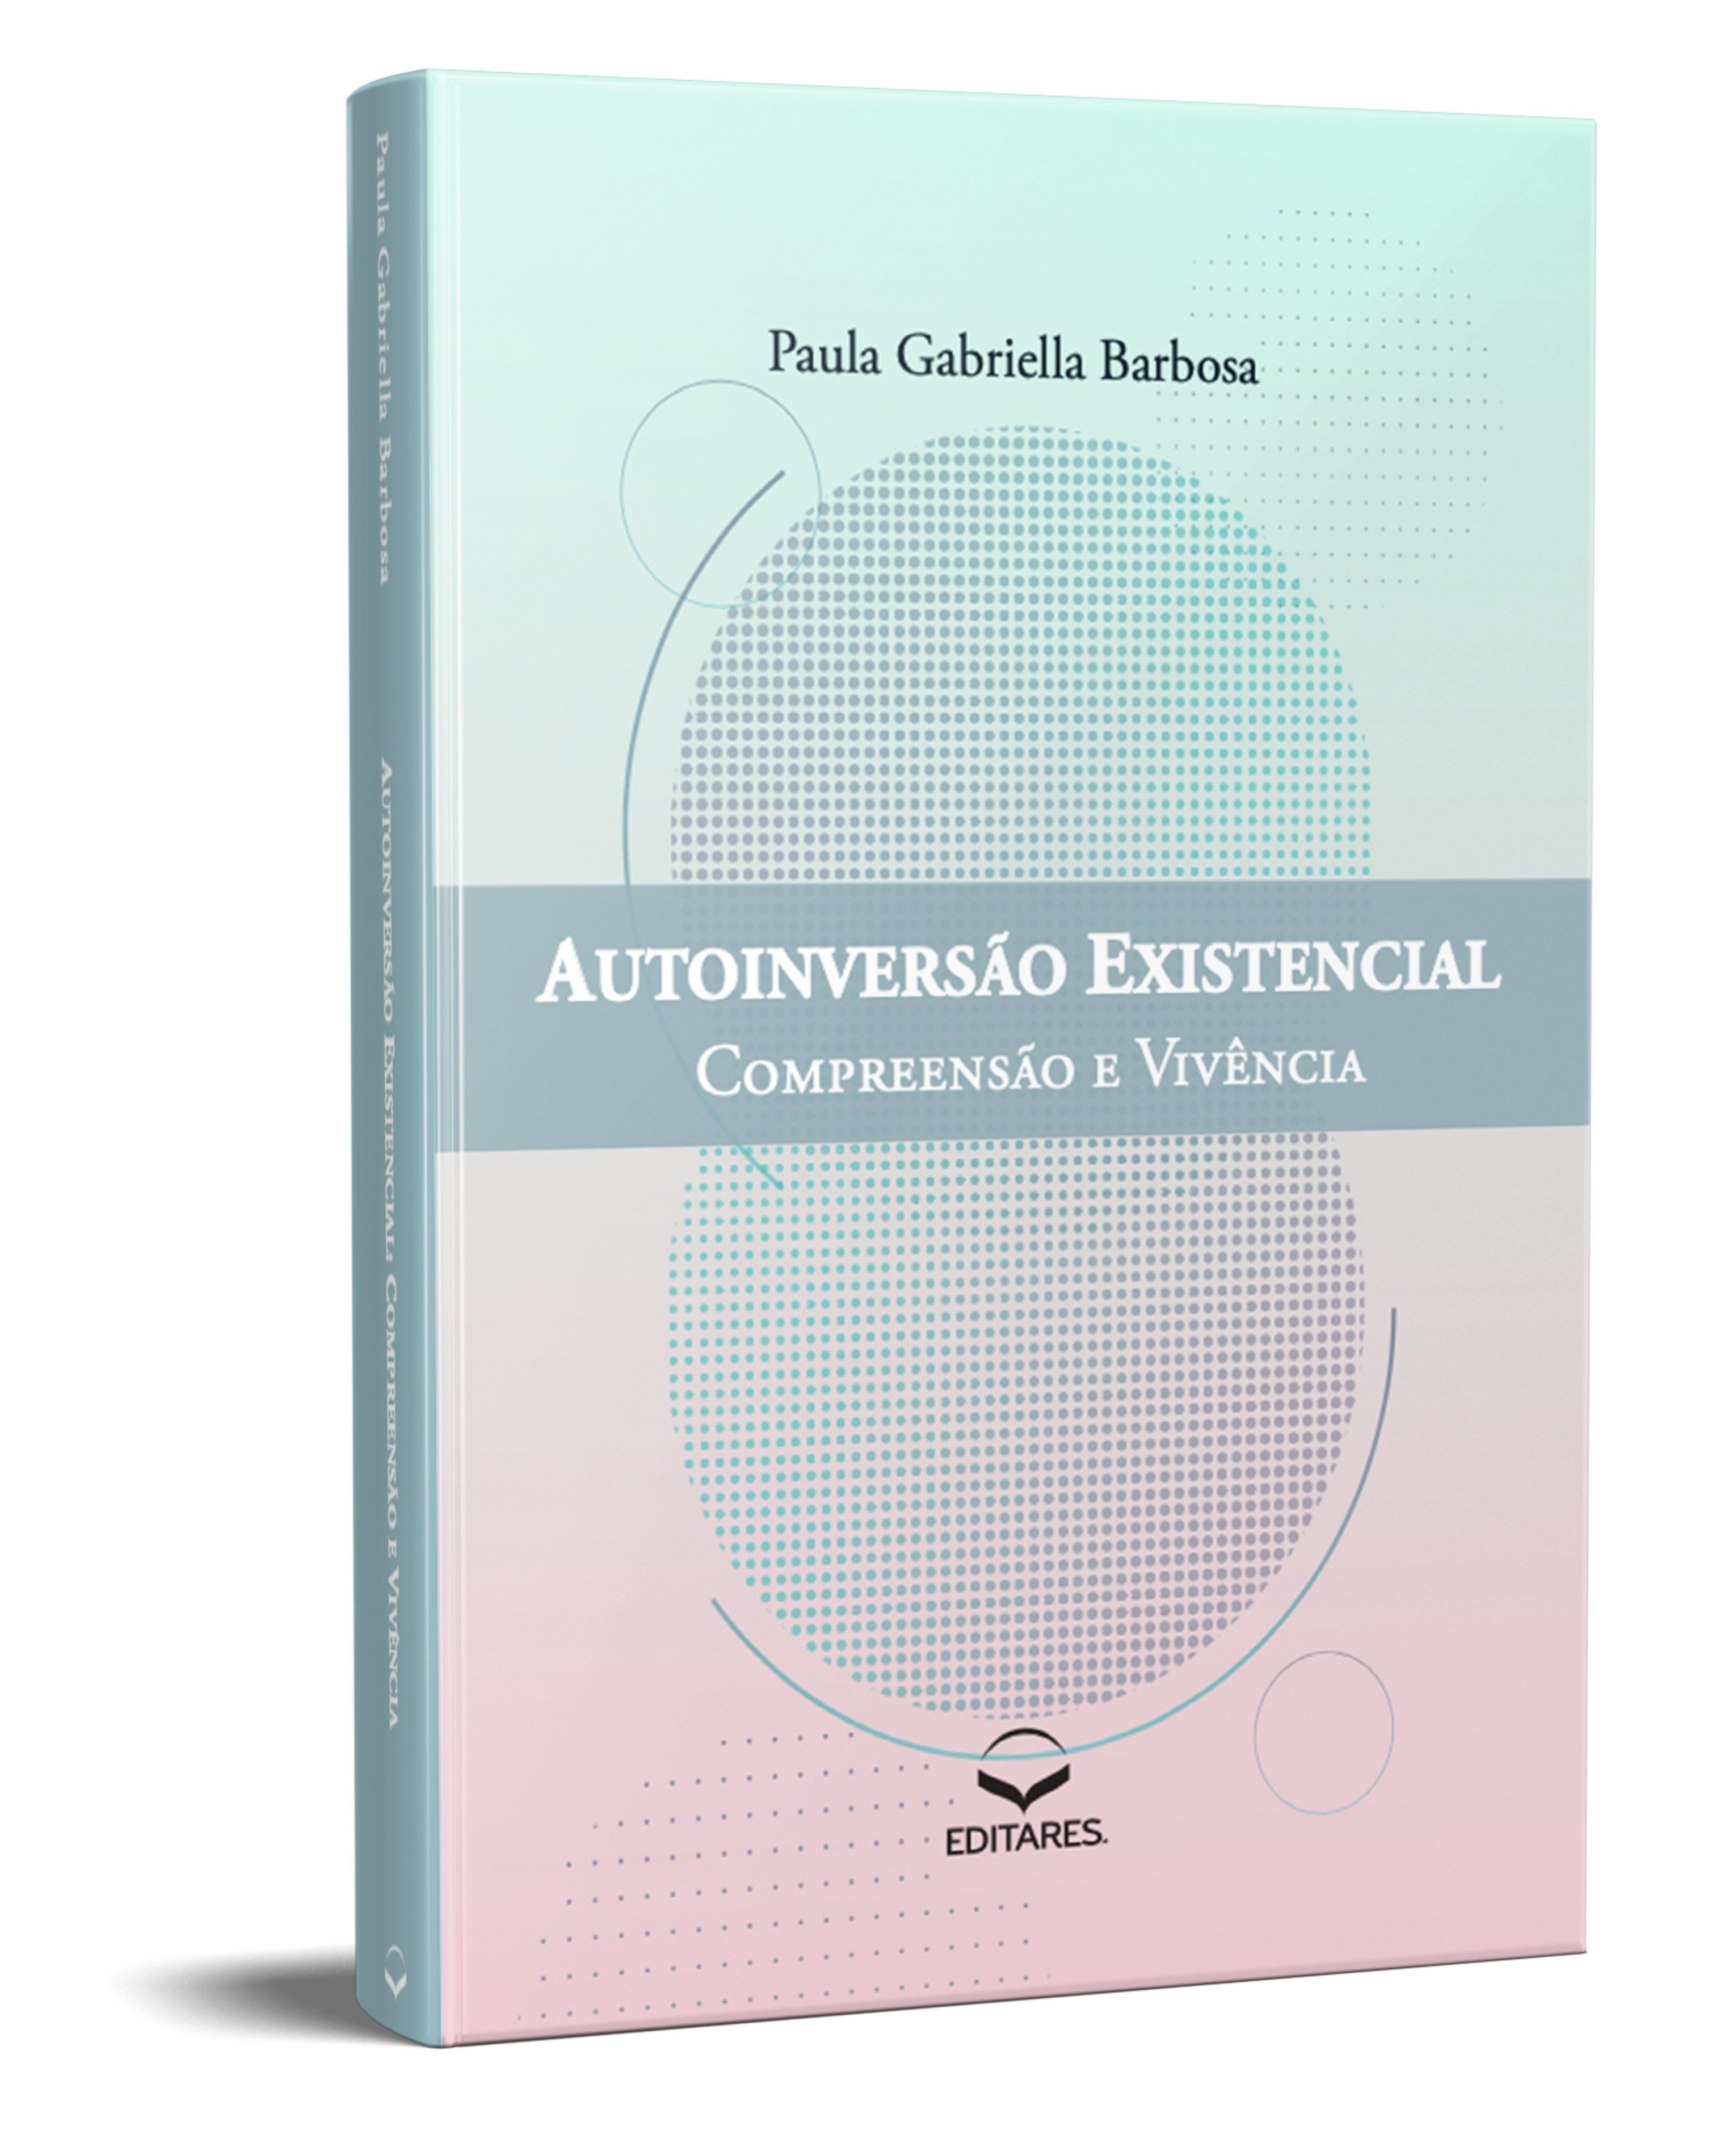
\includegraphics[width=7cm]{articles/entrevista/mockups/Paula.png}
\end{center}


\textbf{1. Qual foi a motivação para a escrita da obra? Por que a definição deste tema para publicação de um livro?}

Minha principal motivação foi compartilhar aprendizados obtidos na aplicação prática da técnica da inversão existencial (invéxis), com o objetivo de auxiliar os leitores na desdramatização dessa proposta evolutiva. O título \textit{Autoinversão Existencial: Compreensão e Vivência} reflete a abordagem intraconsciencial adotada na obra, priorizando os efeitos evolutivos da técnica em detrimento de posturas pro forma. Busquei trazer uma visão mais realista e experiencial, centrada na autorreflexão e no autoenfrentamento cosmoético.

\begin{pullquote}
    ``O título Autoinversão Existencial: Compreensão e Vivência reflete a abordagem intraconsciencial adotada na obra, priorizando os efeitos evolutivos da técnica em detrimento de posturas pró forma.''
\end{pullquote}

\textbf{2. Quais foram as principais percepções, intra e extrafísicas, durante a pesquisa e a escrita da obra? E posterior ao lançamento?}

Durante o processo de escrita, percebi forte presença e amparo de consciências extrafísicas com paravisual e holopensene de matriz oriental, especialmente chinesa. Essa influência se manifestou tanto na leveza da abordagem quanto na clareza reflexiva do conteúdo, favorecendo o desassédio pessoal e o da própria obra. Senti que a escrita ocorreu em conjunto com os amparadores, dada a rapidez e fluidez da redação e editoração. Considero que houve um investimento extrafísico significativo para que o livro se materializasse neste momento evolutivo.

\begin{pullquote}
    ``Considero que houve um investimento extrafísico significativo para que o livro se materializasse neste momento evolutivo.''
\end{pullquote}

\textbf{3. Qual o maior aprendizado com a escrita desta obra?}

O principal aprendizado foi compreender o valor da escrita como forma de posicionamento multidimensional. Através deste livro, consegui expressar de maneira clara meu entendimento sobre a técnica da invéxis, além de assumir um posicionamento mais lúcido diante do meu retrogrupo de base religiosa. Também entendi que, independentemente de onde eu esteja, a obra continuará disponível para as consciências interessadas, mantendo vivas as ideias e experiências compartilhadas.

\textbf{4. O que poderia dizer como incentivo para que mais pesquisadores invistam na publicação de obras conscienciológicas?}

A escrita conscienciológica é uma oportunidade de renovação da autoimagem, além de constituir um posicionamento multidimensional diante do tema abordado. Ao escrever, o pesquisador amplia o alcance assistencial de suas vivências e reciclagens. Publicar é uma forma de fixar marcos na própria trajetória e, ao mesmo tempo, abrir caminhos para outras consciências.
    
    
    \end{multicols}
\end{document}




